\begin{frame}[t,fragile]{テイラー展開によるフォワードモードの計算}
  \begin{itemize}
    %\setlength{\itemsep}{1em}
  \item $x_2 = 0 + \epsilon$, $x_1 = 2$, $x_3 = 1$と表す
  \item 途中の計算を $\epsilon$ の1次まで保存しながら計算
    \begin{itemize}
    \item $v_1 \leftarrow \exp(x_2) = \exp(0 + \epsilon) \approx 1 + \epsilon$
    \item $v_2 \leftarrow x_1 - v_1 = 2 - (1 + \epsilon) = 1 - \epsilon$
    \item $v_3 \leftarrow v_1 \times x_3 = (1 + \epsilon) \times 1 = 1 + \epsilon$
    \item $v_4 \leftarrow v_2 \times v_3 = (1 - \epsilon) \times (1 + \epsilon) \approx 1$
    \item $v_5 \leftarrow v_3 + 1 = (1 + \epsilon) + 1 = 2 + \epsilon$
    \item $f \leftarrow v_4 / v_5 = 1 / (2 + \epsilon) \approx \frac{1}{2} - \frac{1}{4} \epsilon$
    \end{itemize}
  \item $\epsilon$ の係数が微分の値
  \item それぞれの基本演算に対するテイラー展開係数の計算式を用意しておけばよい \ 例)
    \begin{itemize}
    \item $(a + b \epsilon) \times (c + d \epsilon) \approx ac + (ad + bc) \epsilon$
    \item $\exp(a+b\epsilon) \approx \exp(a) + \exp(a) b \epsilon$
    \end{itemize}
  \item 1つの独立変数に関する偏導関数の計算は、関数値$f$の計算コストと同じオーダー → 勾配を計算するにはその$d$倍の計算量が必要

    \vspace*{-17em} \hfill \resizebox{.3\textwidth}{!}{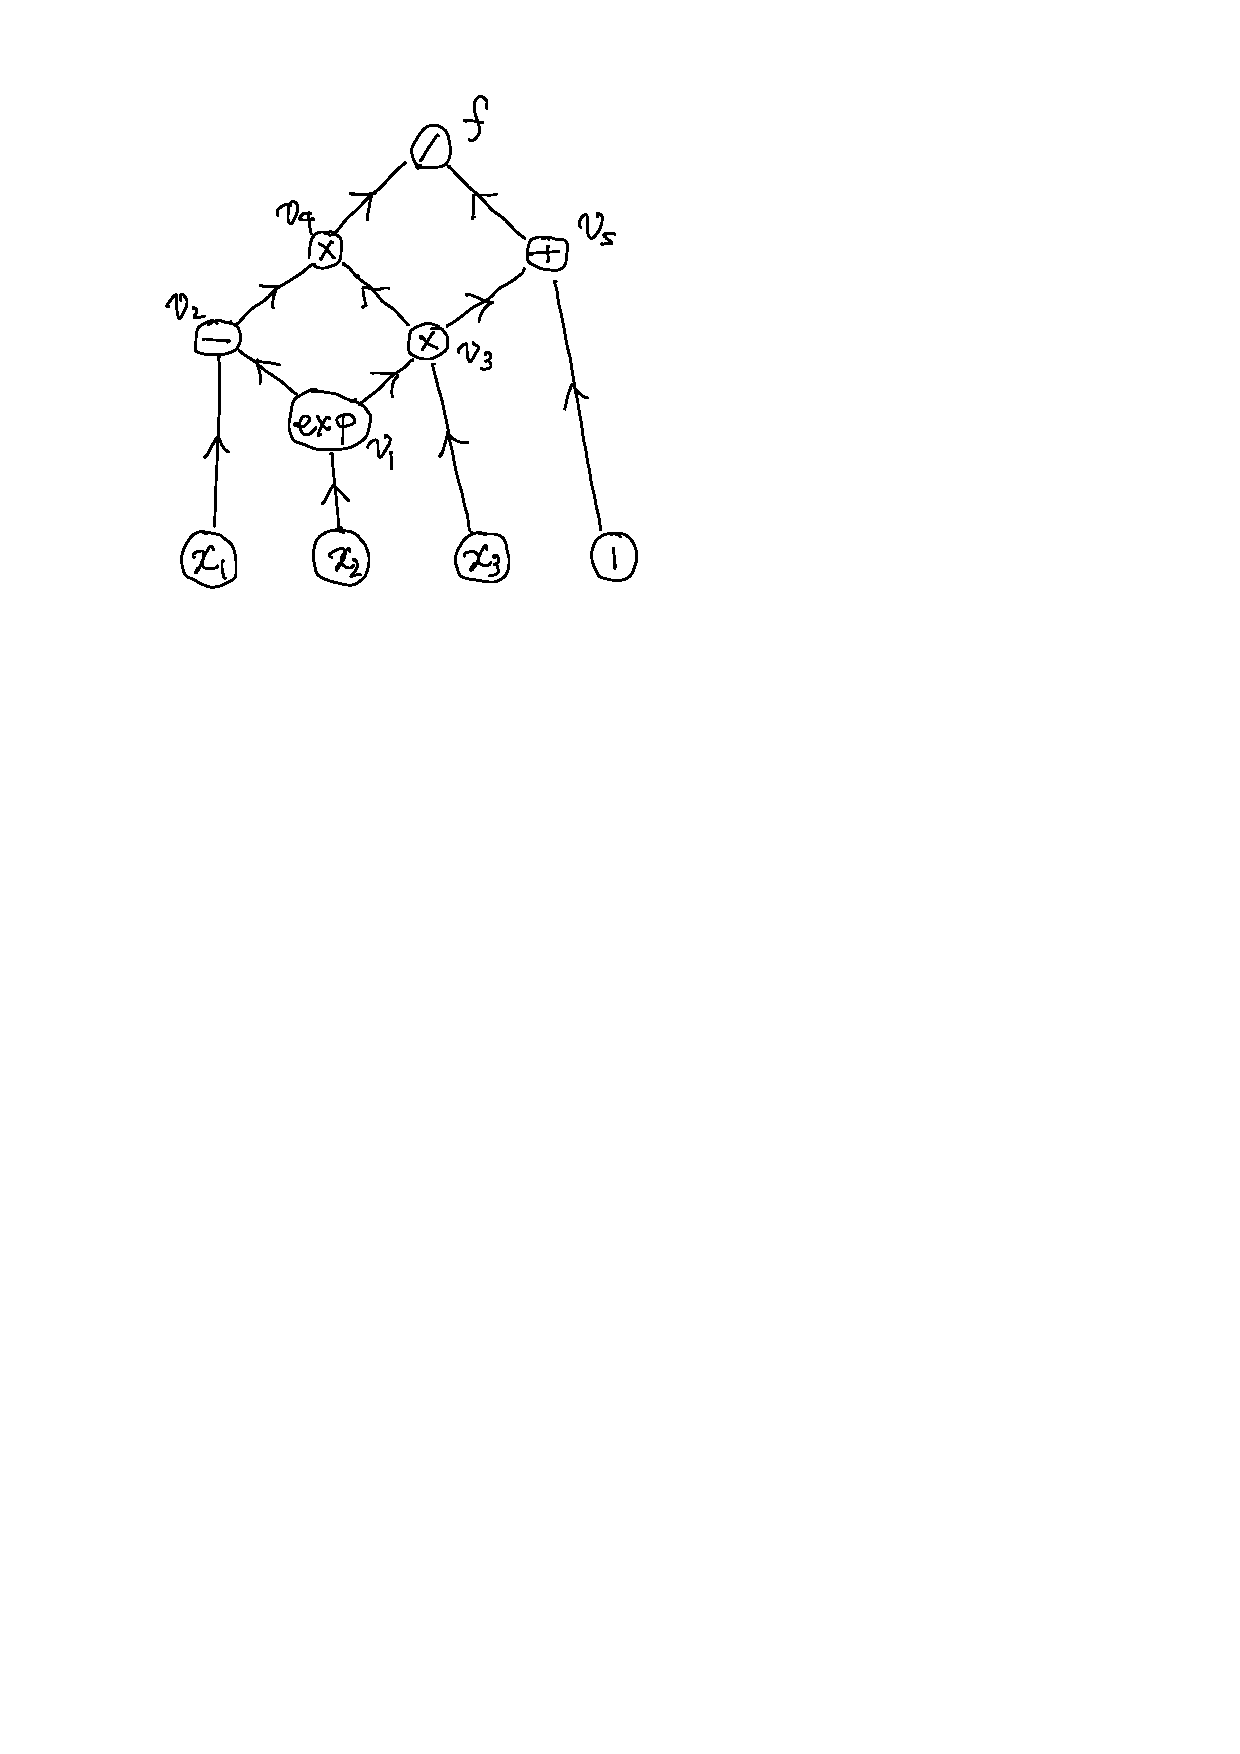
\includegraphics{image/compgraph.pdf}}
  \end{itemize}
\end{frame}
